\documentclass{article}
\usepackage[utf8]{inputenc}
\usepackage{pgf,tikz,pgfplots}
%\usepackage{tikz-3dplot} 
\usepackage{float}
\usepackage{adjustbox}
\usepackage[left=1in, right=1in, top=1in, bottom=1in]{geometry}
\usepackage{mathrsfs}


%\usetikzlibrary{3d}
\usetikzlibrary{arrows,automata,positioning}
\usetikzlibrary{calc}

\pgfplotsset{compat=1.15}


\title{Tikz}
\author{}
\date{} 
 
\begin{document}
\maketitle
\begin{figure}[H]
\centering
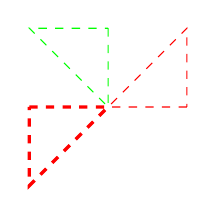
\begin{tikzpicture}
\draw[red, dashed] (1,0) -- (0,0) -- (1,1) -- cycle;
\draw[green, dashed, rotate=90] (1,0) -- (0,0) -- (1,1) -- cycle;
\draw[red, dashed, rotate=180, very thick] (1,0) -- (0,0) -- (1,1) -- cycle;
\end{tikzpicture} 
\caption{Unir puntos, cerrar figuras(cycle), color y  rotar}
\end{figure}

Uso del paquete adjustbox. Uso de perpendiculares y curvaturas
\begin{figure}[H]
\centering
\begin{adjustbox} {width=0.4\textwidth}
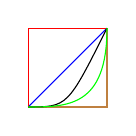
\begin{tikzpicture}
\draw[blue] (0,0) -- (1,1);
\draw[red] (0,0) |- (1,1);
\draw[brown] (0,0) -| (1,1);
\draw[black] (0,0) ..controls(0.5,0) .. (1,1);
\draw[green] (0,0) ..controls(0.5,0) and (1,0) .. (1,1);
\end{tikzpicture} 
\end{adjustbox}
\caption{Uso del paquete adjustbox. Uso de perpendiculares y curvaturas}
\end{figure}



\begin{figure}[H]
\centering
\begin{adjustbox} {width=0.4\textwidth}
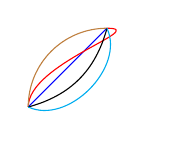
\begin{tikzpicture}
\draw[blue] (0,0) to (1,1);
\draw[red] (0,0) to[out=90, in=0] (1,1);
\draw[brown] (0,0) to[out=90, in=180] (1,1);
\draw[black] (0,0) to[bend right=30] (1,1);
\draw[cyan] (0,0) to[bend right=70] (1,1);
\end{tikzpicture} 
\end{adjustbox}
\caption{manera alterna con to, out para el punto de salida e in para el punto de entrada. Uso de bend right o bend left para curvaturas}
\end{figure}



\begin{figure}[H]
\centering
\begin{adjustbox} {width=0.4\textwidth}
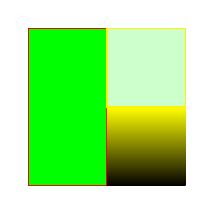
\begin{tikzpicture}
\draw[red,fill=green] (0,0) rectangle (1,2);
\shade[top color=yellow, bottom color=black] (1,0) rectangle (2,1);
\filldraw[fill=green!20!white, draw=yellow] (1,1) rectangle (2,2);
\end{tikzpicture} 
\end{adjustbox}
\caption{dibujar rectangulo con llenado y rectangulo degradado. Usp de filldraw}
\end{figure}



\begin{figure}[H]
\centering
\begin{adjustbox} {width=0.4\textwidth}
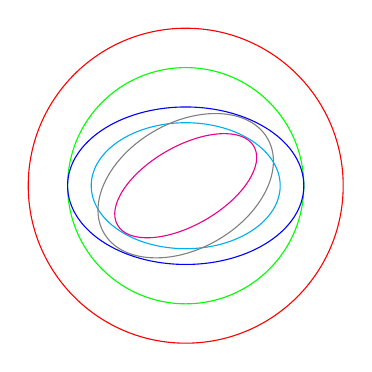
\begin{tikzpicture}
\draw[red] (0,0) circle (2cm);
\draw[green] (0,0) circle [radius=1.5cm];
\draw[cyan] (0,0) circle (1.2cm and 8mm);
\draw[gray, rotate=30] (0,0) circle (1.2cm and 8mm);
\draw[blue] (0,0) circle [x radius=1.5cm, y radius=10mm];
\draw[magenta] (0,0) circle [x radius=1cm, y radius=5mm, rotate=30];
\end{tikzpicture}
\end{adjustbox}
\caption{dibujando circulos y elipsis}
\end{figure}

\begin{figure}[H]
\centering
\begin{adjustbox} {width=0.4\textwidth}
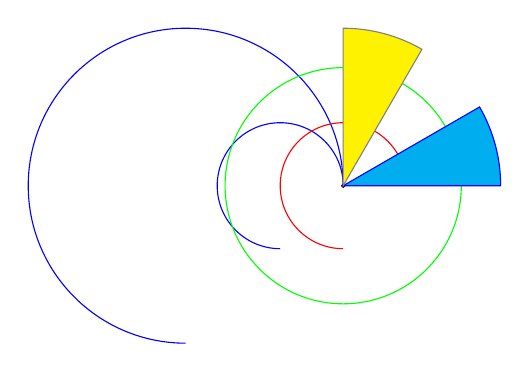
\begin{tikzpicture}
\draw[blue] (0,0) arc (0:270:2cm);
\draw[blue] (0,0) arc (0:270:8mm);
\draw[fill=black] (0,0) circle (0.2mm);
\draw[green] (0,0) circle (1.5);
\draw[red, shift={(8mm,0)}] (0,0) arc (0:270:8mm);
\filldraw[fill=cyan, draw=blue] (0,0) -- (2,0) arc (0:30:2) -- cycle;
\filldraw[fill=yellow, draw=gray, rotate=60] (0,0) -- (2,0) arc (0:30:2) -- cycle;
\end{tikzpicture}
\end{adjustbox}
\caption{sectores circulares, traslados con shift}
\end{figure}


\begin{figure}[H]
\centering
\begin{adjustbox} {width=0.4\textwidth}
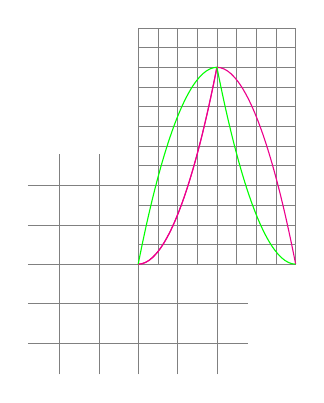
\begin{tikzpicture}
\draw[help lines, step=0.25] (0,0) grid (2,3);
\draw[gray, step=0.5, very thin] (-1.4,-1.4) grid (1.4,1.4);
\draw[magenta] (0,0) parabola (1,2.5);
\draw[magenta] (0,0) parabola (1,2.5) parabola (2,0);
\draw[green] (0,0) parabola[bend at end] (1,2.5) parabola[bend at end] (2,0);
\end{tikzpicture}
\end{adjustbox}
\caption{uso de cuadricula con grid, uso de parabola y concavidad,}
\end{figure}


\begin{figure}[H]
\centering
\begin{adjustbox} {width=0.4\textwidth}
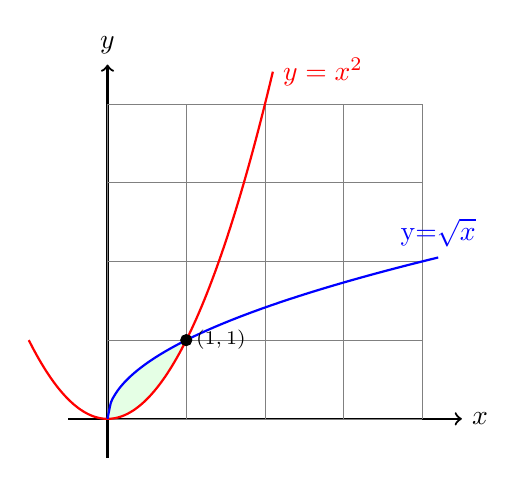
\begin{tikzpicture}
\draw[thick,->] (-0.5,0)--(4.5,0) node[right] {$x$};
\draw[thick,->] (0,-0.5)--(0,4.5) node[above] {$y$}; 
\draw[color=gray,help lines] (0,0) grid (4,4);

\filldraw[draw=none,fill=green!10]
plot [domain=0:1] (\x,{sqrt(\x)})
-- plot [smooth,domain=1:0] (\x,\x^2)
-- cycle;

\draw[domain=-1:2.1, red,samples=100, thick] plot (\x,{\x*\x}) node[right] {$y=x^2$};
\draw[domain=0:4.2, blue, smooth,samples=100, thick] plot (\x,{sqrt(\x)}) node[above] {y=$\sqrt{x}$};

\filldraw[black] (1,1) circle (2pt) node[right] {\scriptsize $(1,1)$};
\end{tikzpicture}
\end{adjustbox}
\end{figure}

\begin{figure}[H]
\centering
\begin{adjustbox} {width=0.4\textwidth}
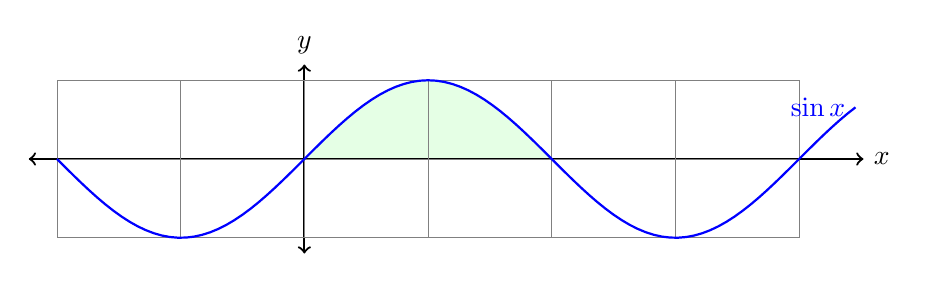
\begin{tikzpicture}

\filldraw[draw=none,fill=green!10]
plot [domain=0:pi] (\x,{sin(\x r)})
-- cycle;

\draw[thick,<->] (-3.5,0)--(7.1,0) node[right] {$x$};
\draw[thick,<->] (0,-1.2)--(0,1.2) node[above] {$y$}; 
\draw[color=gray,help lines, xstep=pi/2] (-pi,-1) grid (2*pi,1);

\draw [domain=-pi:7, blue,samples=100, thick] plot (\x,{sin(\x r)}) node[left] {$\sin x$}; 
\end{tikzpicture}
\end{adjustbox}
\end{figure}


\begin{figure}[H]
\centering
\begin{adjustbox} {width=0.4\textwidth}
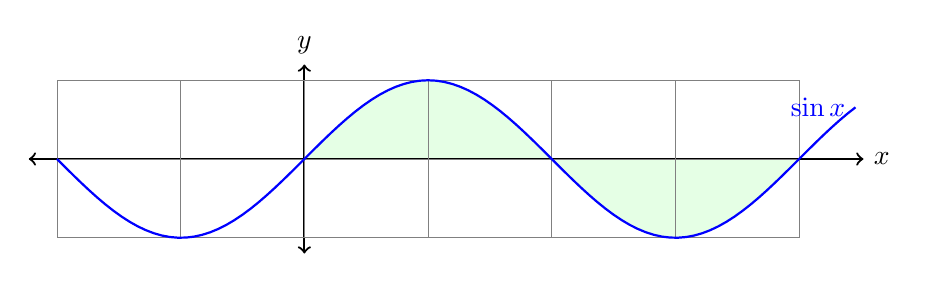
\begin{tikzpicture}

\filldraw[draw=none,fill=green!10]
plot [domain=0:2*pi] (\x,{sin(\x r)})
-- cycle;

\draw[thick,<->] (-3.5,0)--(7.1,0) node[right] {$x$};
\draw[thick,<->] (0,-1.2)--(0,1.2) node[above] {$y$}; 
\draw[color=gray,help lines, xstep=pi/2] (-pi,-1) grid (2*pi,1);

\draw [domain=-pi:7, blue,samples=100, thick] plot (\x,{sin(\x r)}) node[left] {$\sin x$}; 
\end{tikzpicture}
\end{adjustbox}
\end{figure}

\begin{figure}[H]
\centering
\begin{adjustbox} {width=0.4\textwidth}
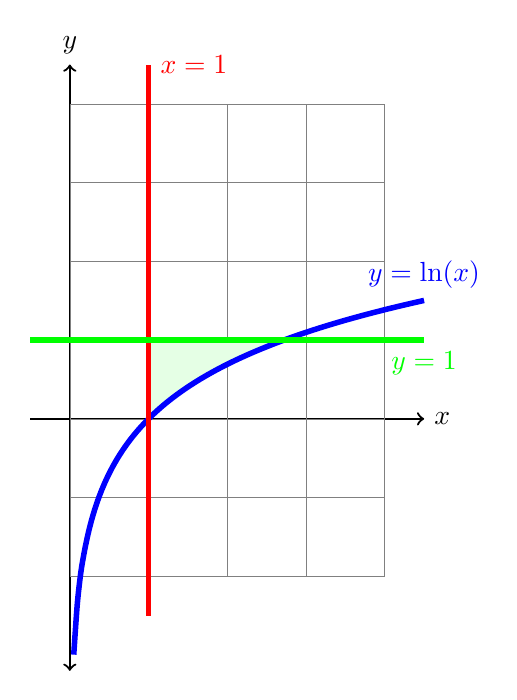
\begin{tikzpicture}
\draw[thick,->] (-0.5,0)--(4.5,0) node[right] {$x$};
\draw[thick,<->] (0,-3.2)--(0,4.5) node[above] {$y$}; 
\draw[color=gray,help lines] (0,-2) grid (4,4);

\filldraw[draw=none,fill=green!10] plot[smooth,domain=1:e](\x,{ln((\x))}) -- (1,1) -- cycle;  

\draw [blue,line width=2.pt,smooth,samples=100,domain=0.05:4.5] plot(\x,{ln((\x))}) node[above] {$y=\ln(x)$};

\draw[red, line width=2, domain=-2.5:4.5]  plot (1, {\x}) node[right] {$x=1$};

\draw[green, line width=2, domain=-0.5:4.5]  plot (\x, {1}) node[below] {$y=1$};
\end{tikzpicture}
\end{adjustbox}
\end{figure}

\begin{figure}[H] 
\centering 
\begin{adjustbox}{width=0.4\textwidth} 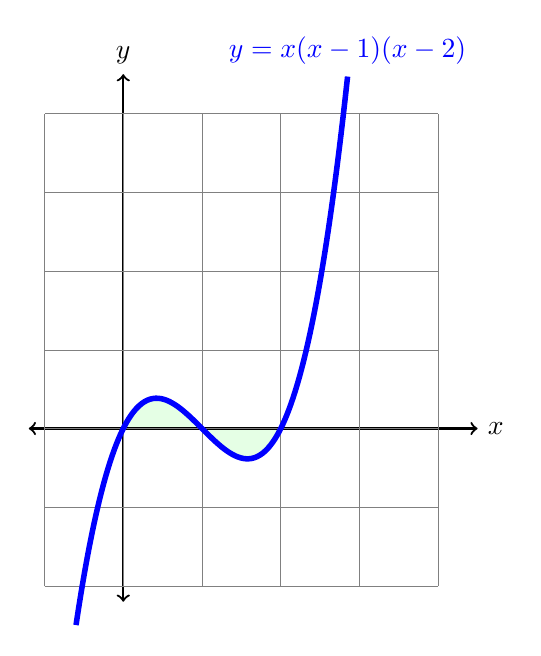
\begin{tikzpicture}

\filldraw[draw=none,fill=green!10] plot[smooth,domain=0:2](\x,{\x*(\x-1)*(\x-2)}) -- cycle;

\draw[thick,<->] (-1.2,0)--(4.5,0) node[right] {$x$};
\draw[thick,<->] (0,-2.2)--(0,4.5) node[above] {$y$};  

\draw[color=gray,help lines] (-1,-2) grid (4,4);

\draw [blue,line width=2.pt,smooth,samples=100,domain=-0.6:2.85] plot(\x,{\x*(\x-1)*(\x-2)}) node[above] {$y=x(x-1)(x-2)$};
\end{tikzpicture} 
\end{adjustbox}
\end{figure}


\begin{figure}[H] 
\centering 
\begin{adjustbox}{width=0.4\textwidth} 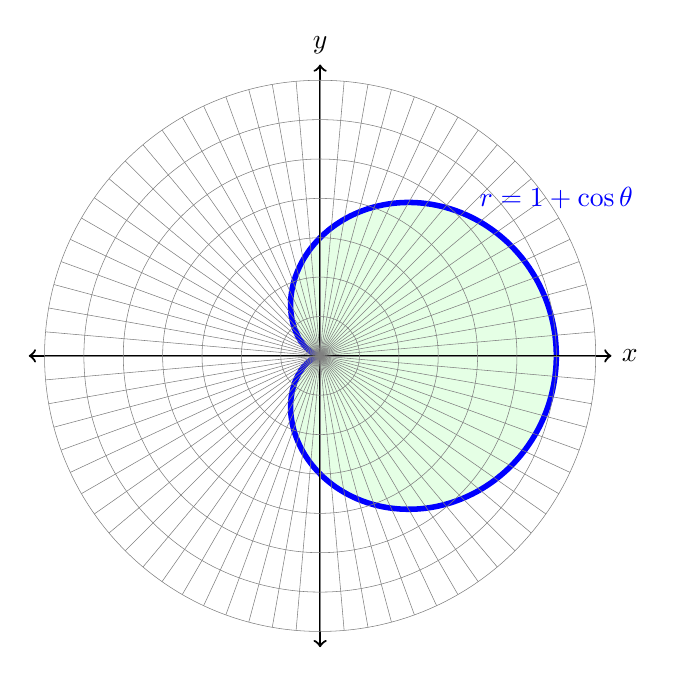
\begin{tikzpicture}

\filldraw[draw=blue,line width=2.pt,fill=green!10,domain=0:3*pi,scale=1.5,samples=500] plot ({deg(\x)}:{1+cos(\x r)});


\draw[thick,<->] (-3.7,0)--(3.7,0) node[right] {$x$};
\draw[thick,<->] (0,-3.7)--(0,3.7) node[above] {$y$};  

\foreach \x in {0,0.5,...,3.5}
\draw[help lines] (0,0) circle(\x);

\foreach \y in {0,5,...,360}
\draw[help lines] (0,0) -- (\y:3.5);

\node[blue] at (3,2) {$r=1+\cos \theta$};
\end{tikzpicture} 
\end{adjustbox}
\end{figure}

\begin{figure}[H] 
\centering 
\begin{adjustbox}{width=0.4\textwidth} 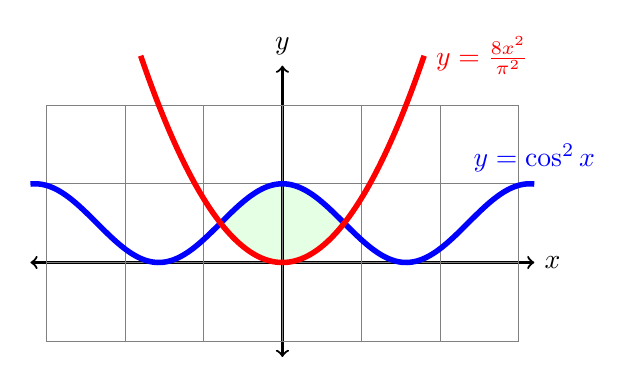
\begin{tikzpicture}

\filldraw[draw=none,fill=green!10] plot[smooth,domain=-pi/4:pi/4] (\x,{8*\x*\x/pi^2}) -- plot[smooth,domain=-pi/4:pi/4] (\x,{(cos(\x r))^2});

\draw[thick,<->] (-3.2,0)--(3.2,0) node[right] {$x$};
\draw[thick,<->] (0,-1.2)--(0,2.5) node[above] {$y$};  

\draw[color=gray,help lines] (-3,-1) grid (3,2);

\draw [blue,line width=2.pt,smooth,samples=100,domain=-3.2:3.2] plot(\x,{(cos(\x r))^2}) node[above] {$y=\cos^2 x$};

\draw [red,line width=2.pt,smooth,samples=100,domain=-1.8:1.8] plot(\x,{8*\x*\x/pi^2}) node[right] {$y=\frac{8x^2}{\pi^2}$};
\end{tikzpicture} 
\end{adjustbox}
\end{figure}

\begin{figure}[H] 
\centering 
\begin{adjustbox}{width=0.4\textwidth} 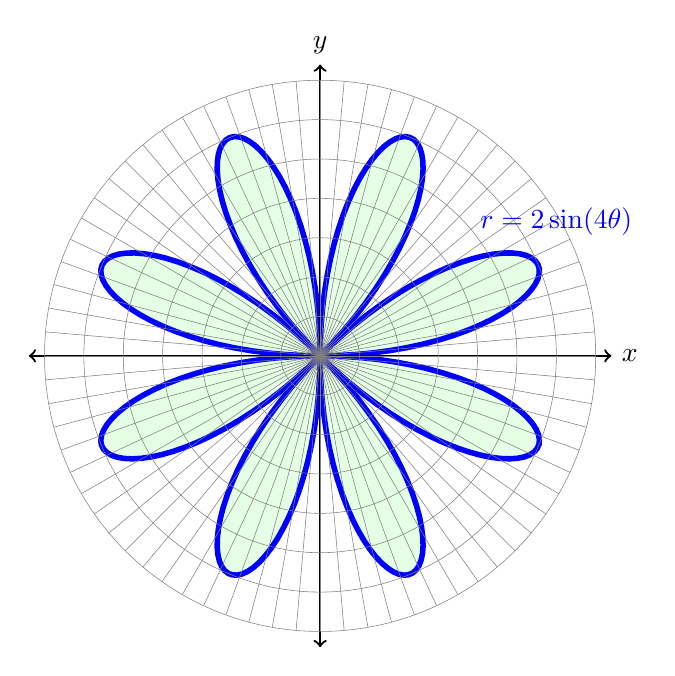
\begin{tikzpicture}

\filldraw[draw=blue,line width=2.pt,fill=green!10,domain=0:3*pi,scale=1.5,samples=500] plot ({deg(\x)}:{2*sin(4*\x r)});

\draw[thick,<->] (-3.7,0)--(3.7,0) node[right] {$x$};
\draw[thick,<->] (0,-3.7)--(0,3.7) node[above] {$y$};  

\foreach \x in {0,0.5,...,3.5}
\draw[help lines] (0,0) circle(\x);

\foreach \y in {0,5,...,360}
\draw[help lines] (0,0) -- (\y:3.5);

\node[blue] at (3,1.7) {$r=2\sin(4\theta)$};
\end{tikzpicture} 
\end{adjustbox}
\end{figure}

\begin{figure}[H] 
\centering 
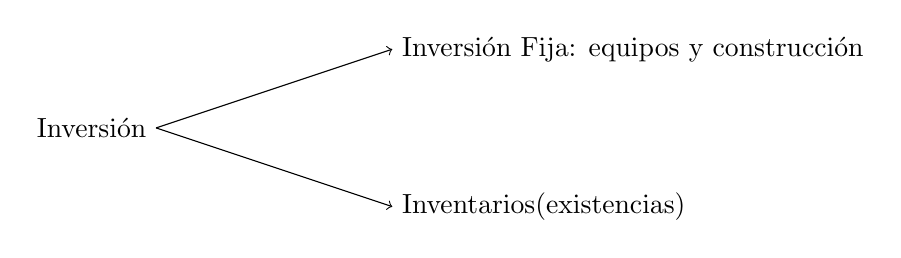
\begin{tikzpicture}
\node[left] at (0,0) {Inversión};
\node[right] at (3,1) {{Inversión Fija: equipos y construcción}}; 
\node[right] at (3,-1) {Inventarios(existencias)}; 
\draw[->] (0,0) -- (3,1);
\draw[->] (0,0) -- (3,-1);
\end{tikzpicture} 
\end{figure}

\begin{figure}[H] 
\centering 
\begin{adjustbox}{width=0.9\columnwidth}
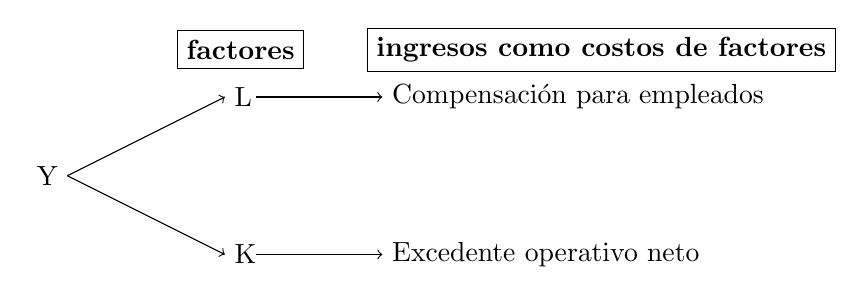
\begin{tikzpicture}
\node[left] at (0,0) {Y};

\node[draw] at (2.2,1.6) {\textbf{factores}};
\node[right] at (2,1) {L}; 
\node[right] at (2,-1) {K};


\node[draw, right] at (3.8,1.6) {\textbf{ingresos como costos de factores}};
\node[right] at (4,1) {Compensación para empleados};
\node[right] at (4,-1) {Excedente operativo neto};

\draw[->] (0,0) -- (2,1);
\draw[->] (0,0) -- (2,-1);
\draw[->] (2.4,1) -- (4,1);
\draw[->] (2.4,-1) -- (4,-1);
\end{tikzpicture}
\end{adjustbox}
\end{figure}

\begin{figure}[H]
\centering
\begin{adjustbox} {height=0.4\textheight}
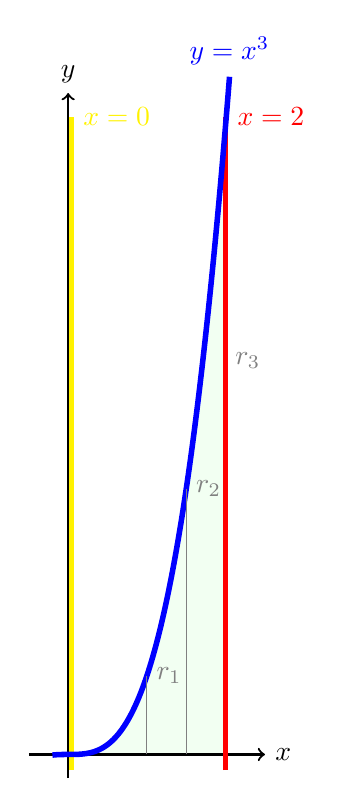
\begin{tikzpicture}

\filldraw[draw=none,fill=green!5] (0,0) -- plot[domain=0:2,smooth,samples=100] (\x,{\x^3)}) -- (2,0) --cycle; 


\draw[thick,->] (-0.5,0)--(2.5,0) node[right] {$x$};
\draw[thick,->] (0,-0.3)--(0,8.4) node[above] {$y$}; 


\draw[yellow, line width=2pt, domain=-0.2:8.1]  plot (0.04, {\x}) node[right] {$x=0$};

\draw[red, line width=2pt, domain=-0.2:8.1]  plot (2, {\x}) node[right] {$x=2$};

\draw [blue,line width=2.pt,smooth,samples=100,domain=-0.2:2.05] plot(\x,{\x^3)}) node[above] {$y=x^3$};

\node[black!50, right] at (2,5) {$r_3$};

\draw[black!50] (1,0)--(1,1) node[right] {$r_1$};

\draw[black!50] (1.5,0)--(1.5,1.5^3) node[right] {$r_2$};

\end{tikzpicture}
\end{adjustbox}
\end{figure}


\begin{figure}[H]
\centering
\begin{adjustbox} {width=0.6\textwidth}
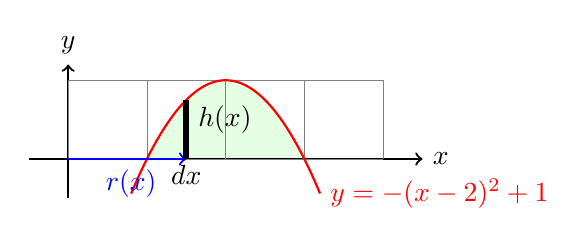
\begin{tikzpicture}

\filldraw[draw=none,fill=green!10] plot [domain=1:3] (\x,{-(\x-2)^2+1})--cycle;

\draw[thick,->] (-0.5,0)--(4.5,0) node[right] {$x$};
\draw[thick,->] (0,-0.5)--(0,1.2) node[above] {$y$}; 
\draw[color=gray,help lines] (0,0) grid (4,1);

\draw [domain=0.8:3.2, red,samples=100, thick] plot (\x,{-(\x-2)^2+1}) node[right] {$y=-(x-2)^2+1$};

\draw[blue,thick,->] (0,0)-- (0.8,0) node[below] {$r(x)$} -- (1.5,0);
\draw[black,line width=2pt] (1.5,0)--(1.5,0.5) node[right] {$h(x)$}-- (1.5,0.75);

\node at (1.5,-0.2) {$dx$}; 
\end{tikzpicture}
\end{adjustbox}
\end{figure}


\begin{figure}[H]
\centering
\begin{adjustbox} {width=0.4\textwidth}
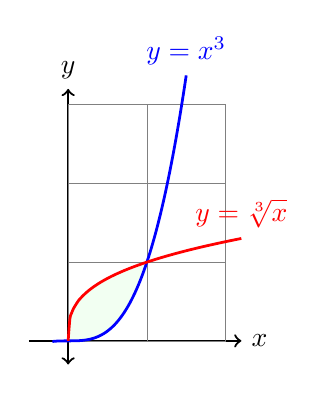
\begin{tikzpicture}

\filldraw[draw=none,fill=green!5] plot[domain=0:1,smooth,samples=100] (\x,{\x^3)}) -- plot[domain=1:0,smooth,samples=100] (\x,{(\x)^(1/3)}); 

\draw[thick,->] (-0.5,0)--(2.2,0) node[right] {$x$};
\draw[thick,<->] (0,-0.3)--(0,3.2) node[above] {$y$};
\draw[help lines] (0,0) grid (2,3);

\draw [blue,line width=1.pt,smooth,samples=100,domain=-0.2:1.5] plot(\x,{\x^3)}) node[above] {$y=x^3$};

\draw [red,line width=1.pt,smooth,samples=100,domain=0:2.2] plot(\x,{(\x)^(1/3)}) node[above] {$y=\sqrt[3]{x}$};
\end{tikzpicture}
\end{adjustbox}
\end{figure}

\begin{figure}[H]
\centering
\begin{adjustbox} {width=0.4\textwidth}
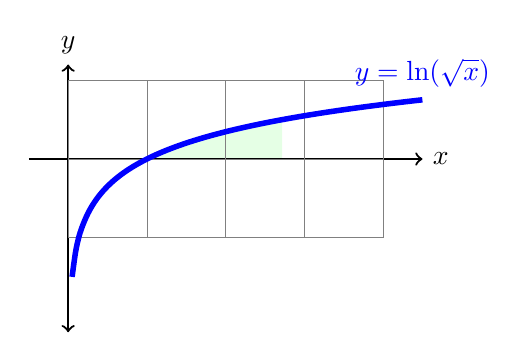
\begin{tikzpicture}

\filldraw[draw=none,fill=green!10] plot[smooth,domain=1:e](\x,{ln((\x^0.5))}) -- (e,0) -- cycle;  

\draw[thick,->] (-0.5,0)--(4.5,0) node[right] {$x$};
\draw[thick,<->] (0,-2.2)--(0,1.2) node[above] {$y$}; 
\draw[color=gray,help lines] (0,-1) grid (4,1);

\draw [blue,line width=2.pt,smooth,samples=100,domain=0.05:4.5] plot(\x,{ln((\x^0.5))}) node[above] {$y=\ln(\sqrt{x})$};

\end{tikzpicture}
\end{adjustbox}
\end{figure}


\begin{figure}[H] 
\centering 
\begin{adjustbox} {height=0.4\textheight} 
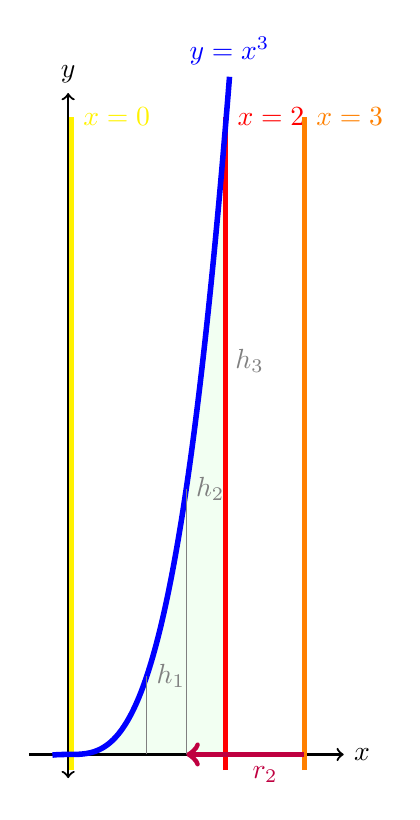
\begin{tikzpicture}

\filldraw[draw=none,fill=green!5] (0,0) -- plot[domain=0:2,smooth,samples=100] (\x,{\x^3)}) -- (2,0) --cycle; 

\draw[thick,->] (-0.5,0)--(3.5,0) node[right] {$x$}; 
\draw[thick,<->] (0,-0.3)--(0,8.4) node[above] {$y$}; 

\draw[yellow, line width=2pt, domain=-0.2:8.1]  plot (0.04, {\x}) node[right] {$x=0$};
\draw[red, line width=2pt, domain=-0.2:8.1]  plot (2, {\x}) node[right] {$x=2$};
\draw [blue,line width=2.pt,smooth,samples=100,domain=-0.2:2.05] plot(\x,{\x^3)}) node[above] {$y=x^3$};

\draw[orange, line width=2pt, domain=-0.2:8.1]  plot (3, {\x}) node[right] {$x=3$};

\draw[purple, line width=2pt,->] (3,0) --(2.5,0) node[below]{$r_2$}-- (1.5,0);

\node[black!50, right] at (2,5) {$h_3$};
\draw[black!50] (1,0)--(1,1) node[right] {$h_1$};
\draw[black!50] (1.5,0)--(1.5,1.5^3) node[right] {$h_2$};
\end{tikzpicture} 
\end{adjustbox} 
\end{figure}



\begin{figure}[H] 
\centering 
\begin{adjustbox} {height=0.4\textheight} 
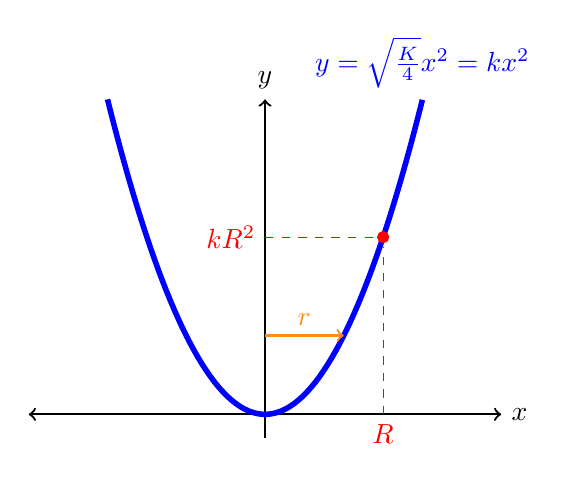
\begin{tikzpicture}

\draw[thick,<->] (-3,0)--(3,0) node[right] {$x$}; 
\draw[thick,->] (0,-0.3)--(0,4) node[above] {$y$}; 

\draw [blue,line width=2.pt,smooth,samples=100,domain=-2:2] plot(\x,{(\x)^2}) node[above] {$y=\sqrt{\frac{K}{4}}x^2=kx^2$};

\node[below,red] (A) at (1.5,0) {$R$};
\node[left,red] (B) at (0,2.25) {$kR^2$};
\node (C) at (1.5,2.25) {};
\filldraw[black,red]  (C) circle (2pt);

\draw[dashed,red] (A) -- (C); 
\draw[dashed,red] (B) -- (C); 

\draw [orange!90,line width=0.8pt,->] (0,1) -- (0.5,1) node[above]{$r$}-- (1,1); 
\end{tikzpicture} 
\end{adjustbox} 
\end{figure}

\begin{figure}[H]
\centering
\begin{adjustbox} {width=\columnwidth}
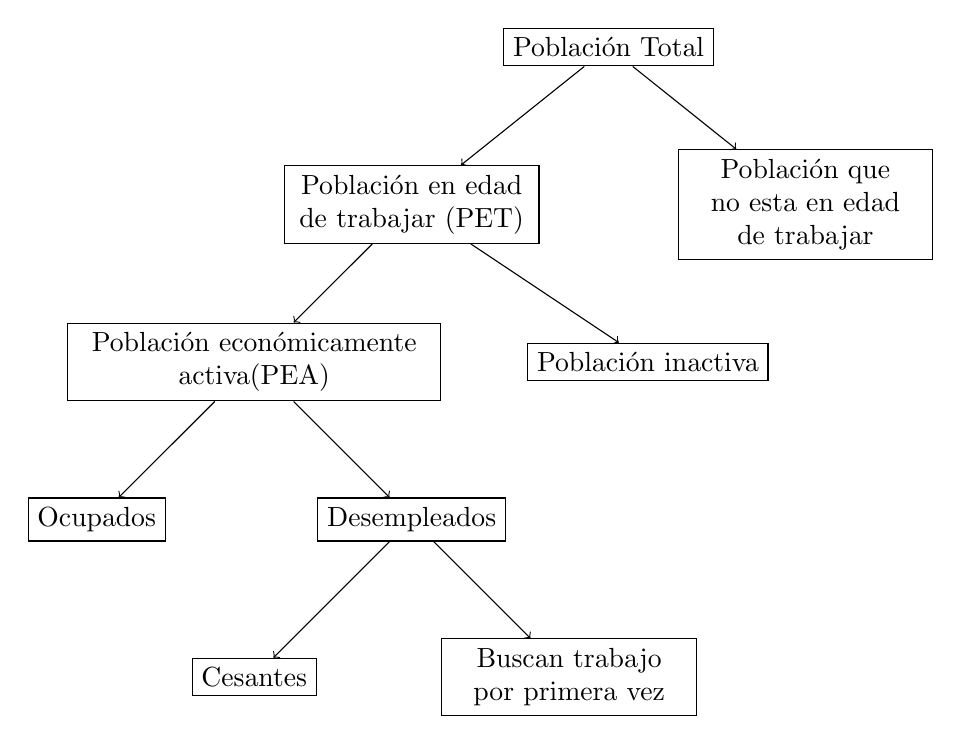
\begin{tikzpicture}

\node[draw] (A) at (8.5,10) {Población Total};

\node[draw, text width = 3cm, text centered] (B) at (6,8) {Población en edad de trabajar (PET)};
\node[draw, text width = 3cm, text centered] (C) at  (11,8) {Población que no esta en edad de trabajar};

\node[draw, text width = 4.5cm, text centered] (E) at (4,6){Población económicamente activa(PEA)};
\node[draw, text centered] (D) at (9,6){Población inactiva};

\node[draw, text centered] (F) at (2,4){Ocupados};
\node[draw, text centered] (G) at (6,4){Desempleados};

\node[draw, text centered] (H) at (4,2){Cesantes};
\node[draw, text width = 3cm, text centered] (I) at (8,2){Buscan trabajo por primera vez};

\draw[->] (A) -- (B);
\draw[->] (A) -- (C);

\draw[->] (B) -- (D);
\draw[->] (B) -- (E);

\draw[->] (E) -- (F);
\draw[->] (E) -- (G);

\draw[->] (G) -- (H);
\draw[->] (G) -- (I);

\end{tikzpicture}
\end{adjustbox}
\end{figure}

\begin{figure}[H]
\centering
\begin{adjustbox} {width=\columnwidth}
\begin{tikzpicture}
\draw[->] (-2,0) -- (5,0) node[right] {$x$};
\draw[->] (0,-2) -- (0,5) node[above] {$y$};

\draw[red, <->]  (-2,-1) -- (3,4) node[right] {$L_1: A_1x+B_1y+C_1=0$};
\draw[blue, <->] (4,-1)-- (-2,4)  node[left] {$L_2: A_2x+B_2y+C_2=0$};

\begin{scope}
\path[clip]  (5,0) --(2.8,0)--(-2,4);
\fill[blue, opacity=0.5, draw=black] (2.8,0) circle (1.5mm);
\node[blue] at ($(2.8,0)+(60:3.5mm)$) {$\theta_1$};
\end{scope}

\begin{scope}
\path[clip]  (5,0) --(-1,0)-- (3,4);
\fill[red, opacity=0.5, draw=black] (-1,0) circle (2.5mm);
\node[red] at ($(-1,0)+(20:5.5mm)$) {$\theta_2$};
\end{scope}
\end{tikzpicture}
\end{adjustbox}
\end{figure}

\begin{figure}[H]
\centering
\begin{adjustbox} {width=\columnwidth}
\begin{tikzpicture}

\coordinate (O) at (0,0); 
\coordinate[label= left:$\overline{C}$] (C) at (0,3);

\draw[->] (O) -- (8,0) node[right] {$Y^d$};
\draw[->] (O) -- (0,8) node[above] {$C$};

\draw[black]  (C) -- (7.2,7.5) node[right] {$C=\overline{C}+cY^d$};

\coordinate (E1) at (2,4.25);
\coordinate[label= left:$C_1$,blue] (C1) at (0,4.25);
\coordinate[label= below:$Y^d_1$,blue] (Y1) at (2,0);
\draw[dashed] (C1)--(E1);
\draw[dashed] (Y1)--(E1);
\draw[red,dashed] (O)--node[pos=.5,fill=white,inner sep=1pt]{$\mbox{PMe}C_1$} (E1);

\coordinate (E2) at (6,6.75);
\coordinate[label= left:$C_2$,blue] (C2) at (0,6.67);
\coordinate[label= below:$Y^d_2$,blue] (Y2) at (6,0);
\draw[dashed] (C2)--(E2);
\draw[dashed] (Y2)--(E2);
\draw[red,dashed] (O)--node[pos=.5,fill=white,inner sep=1pt]{$\mbox{PMe}C_2$} (E2);
\end{tikzpicture}
\end{adjustbox}
\end{figure}





\end{document}